\chapter{The Single Skill That Built His \$100M Year Business}

This chapter reads a School of Hard Knocks interview, with curation by LazyingArt LLC, as a compact lecture on portable commercial skill. Johnny Anton's recurring claim is that sales is not simply a role inside a company. It is a transportable craft that can survive poverty, unstable markets, and even the loss of capital. The mathematical structure here is therefore schematic rather than literal. We use equations to preserve the lecture's causal order: failure must be de-dramatized, imagination must be disciplined, action must be reviewed, and scale depends not only on effort but on borrowed pattern recognition.

\section{The Opening Thesis: A Portable Commercial Skill}

The lecture opens in documentary mode rather than in direct instruction. Anton is introduced as someone who helped scale multiple businesses to over nine figures in revenue, and that credential is immediately set against a harsher background: an immigrant family from Iraq, poverty in Detroit, and two years of homelessness. The point of the montage is not sentimental. It is to establish the asymmetry between unstable conditions and a comparatively stable skill.

That is why the opening promise is stated in such strong terms. Markets can fall, crypto can fall, fraud can appear, and yet the person who can sell a high-demand offer remains useful. Before we are given habits, we are given a thesis: some forms of commercial ability travel better than wealth itself.

The montage also plants two later ideas in advance. Anton is presented not only as a closer but as a builder of systems, and the opening teaser names two claims that the chapter will eventually justify: first, that strong leadership depends on a strong product; second, that the movement from eight figures toward nine depends heavily on recruiting and fundraising. The lecture therefore begins with breadth, and only afterward narrows into method.

\section{Failure, Significance, and the Compounding of Time}

\subsection{Question \& Answer}

The first direct question asks what Anton would tell his younger self. The answer is deliberately simple: fail faster, and do not make the failure mean too much. This is the first real update rule in the lecture. It removes emotional drag from experimentation.

We can write the rule schematically as
\begin{equation}
\text{Failure} + \text{Learning} + \text{Time} \to \text{Compounded Improvement}.
\end{equation}

The crucial term is not merely \text{Failure}; it is \text{Time}. Anton's complaint is that people convert small reversals into existential verdicts. Once failure is over-signified, experimentation slows down, and the compounding of learning is interrupted. The lecture then widens this point by way of a cultural example. Anton invokes Israel and says, in effect, that a high-output entrepreneurial culture teaches children to fail forward intelligently and to learn from mistakes without attaching catastrophic meaning to them.

We should state that cautiously: this is Anton's example and Anton's interpretation. But its pedagogical function is unmistakable. The lecture wants to move us from theatrical disappointment to repeated trial. Only after that emotional obstruction is removed can it ask for habit, practice, and structure.

The transition here is important. The lecturer does not ask for business tactics immediately. He first asks for a way of handling error. In that sense the first half of the chapter is not about external mechanics at all. It is about clearing the mind so that later mechanics can become usable.

\section{Step One: Meditation, Imagination, and Reconditioning the Mind}

Once failure has been stripped of excessive significance, the interviewer asks for the habits behind Anton's success. The answer begins inwardly. The first habit is not a script, a funnel, or a hiring plan. It is meditation. Anton describes it as reconditioning the mind, opening the subconscious to the conscious, and removing limitations inherited from the past.

\begin{figure}[ht]
\centering

\includegraphics[width=0.82\textwidth]{lecture_108_figure_02.png}
\caption{The lecture's first numbered habit as it appears on screen: meditating every day.}
\end{figure}

The visible editorial label is itself worth preserving because it fixes the lecture's sequence:
\begin{equation}
\text{STEP 1: MEDITATING EVERYDAY}.
\end{equation}

The figure does not contain a derivation. What it does contain is the numbering, and the numbering matters. Anton is no longer speaking in generalities. He is building an ordered architecture.

He then expands meditation into a larger claim about imagination. Every realized thing begins as something not yet present in the material world. The Disney example is used precisely because it sounds implausible on first hearing: a fictitious amusement park, cartoon characters, adults and children moving through that invented world, and large amounts of capital requested before the object exists. Anton says that around 150 bankers said no, that the initial number was about \$5 million, and that the final cost reached about \$15 million. The anecdote gives entrepreneurial mass to what might otherwise sound like empty manifestation talk.

The lecture's causal line may be written as
\begin{equation}
\text{Imagination} \to \text{Thought} \to \text{Action} \to \text{Material Result}.
\end{equation}

This is a careful reconstruction rather than a literal board formula, but it preserves the order of the argument. One must first hold a form in mind that is not yet possessed. Meditation is then presented as the daily discipline by which possibility is made durable enough to guide behavior.

\paragraph{Anecdote.}
Anton says he has meditated consistently for over six years, and that one early model came from wrestling camp, where athletes meditated every day on winning the state championship.

\paragraph{Claim.}
The first habit is a daily inner practice meant to draw in abundance and possibility while removing old limitations.

\paragraph{Mechanism.}
New information cannot stabilize inside an unchanged identity. Meditation is presented as the mechanism that reconditions the receiving structure before further tactics are added.

At this point the lecture has established its first step: we begin by changing the mind that is doing the acting. Only then do we turn outward.

\section{Step Two and Step Three: Feedback and Pattern Recognition}

The lecture now leaves the interior and becomes operational. Anton's second habit is consistent action plus disciplined review. His third is the decision to pay for access to people who already have the result.

We may summarize the second step by writing
\begin{equation}
\text{Action}_t + \text{Documentation}_t \to \text{Feedback Loop} \to \text{Pattern Recognition}.
\end{equation}

Anton's concrete example is the end-of-day report for the sales team. Who was contacted? What was the result? What worked? What failed? But again he adds a more discriminating layer. One must not track only what was said. One must also track who one was being behind the words. This leads to his sharpest compressed proposition:
\begin{equation}
\text{Context} > \text{Content}.
\end{equation}

The lecture's logic here is best seen through a tiny worked example. Two people may be given the same literal script, and yet their results differ. In that case the text alone cannot explain the outcome:
\begin{align}
\text{Content}_A &= \text{Content}_B,\\
\text{Context}_A &\neq \text{Context}_B,\\
\Rightarrow \text{Result}_A &\neq \text{Result}_B.
\end{align}

This is not mathematical physics, but it is a genuine analytic move. Hold the verbal surface fixed; vary the underlying state, framing, and delivery; observe that the result moves. The lecture wants us to stop attributing performance entirely to the visible script.

Anton later states the reduction even more plainly. Everything comes down to stimulus and response, input and output:
\begin{equation}
\text{Stimulus} \to \text{Response}, \qquad \text{Input} \to \text{Output}.
\end{equation}

That line belongs here because it explains why documentation matters. If the world is continually giving responses to what we put out, then unrecorded time is lost data. We can therefore write the daily update in a slightly more explicit form:
\begin{align}
\text{Log}_t &= (\text{contacts},\text{outcomes},\text{working patterns},\text{failed patterns},\text{context}),\\
\text{Review}(\text{Log}_t) &\to \text{Pattern Recognition}_{t+1},\\
\text{Pattern Recognition}_{t+1} &\to \text{Action}_{t+1}.
\end{align}

He reaches for athletics to make the same point. Winners do not merely enjoy the fact of a win; they review the game to see what actually happened inside it. That is the role of the sports analogy even where the transcript becomes noisy. A result, by itself, is not yet an explanation.

The third step extends this logic outward. If pattern recognition is valuable, the fastest way to obtain it is not always to invent it ourselves. We may buy compressed learning from people who already possess it:
\begin{equation}
\text{Proven Models} + \text{Paid Access} \to \text{Transferred Pattern Recognition}.
\end{equation}

\begin{figure}[ht]
\centering
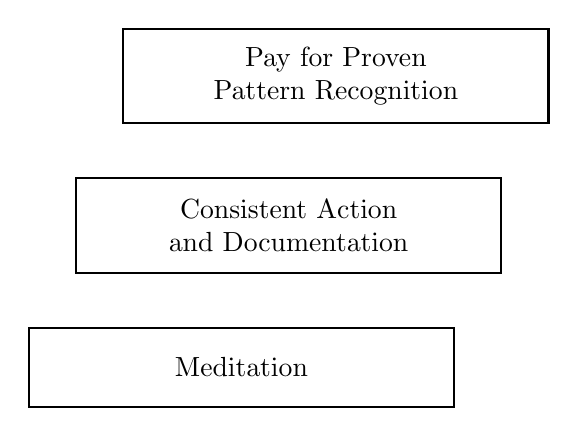
\begin{tikzpicture}
\draw[thick] (0,0) rectangle (5.4,1.0);
\node[align=center] at (2.7,0.5) {Meditation};

\draw[thick] (0.6,1.7) rectangle (6.0,2.9);
\node[align=center] at (3.3,2.3) {Consistent Action\\and Documentation};

\draw[thick] (1.2,3.6) rectangle (6.6,4.8);
\node[align=center] at (3.9,4.2) {Pay for Proven\\Pattern Recognition};
\end{tikzpicture}
\caption{A compact reconstruction of the lecture's three-step architecture.}
\end{figure}

The later recap---``What did I say?''---is not decorative repetition. It is a hinge. The lecture is closing one block of thought: recondition the mind, review action, borrow proven patterns. Only after that compression does it pivot to a different question, namely why intelligent people still sabotage themselves when they begin to build.

\section{Founder Ego and the Cost of the Old Identity}

\subsection{Question \& Answer}

The next question concerns starting a business, and Anton answers with unusual bluntness: ego is not your friend. The lecture has just spent time explaining how to learn quickly. It now asks why that learning so often fails to take root.

The anecdote is concrete. Anton recalls his former boss, Paul, asking whether he really wanted to give up roughly \$500{,}000 in 100\% commission sales income. That income, Paul points out, came without marketing burden, delivery risk, hiring burden, operational burden, or finance burden. Anton's younger self believed the next move would be easy. He had helped scale a company, built training and action plans, refined sales processes and advanced scripting, and felt, at twenty-four, that founder-level success should follow almost automatically.

\paragraph{Anecdote.}
He describes his younger posture as arrogance: previous competence was taken as sufficient proof that every next level would yield to the same will.

\paragraph{Claim.}
The real obstruction is not lack of intelligence or lack of work ethic. It is attachment to the old identity.

\paragraph{Mechanism.}
The ego wants authorship, control, and proof of superiority. For that reason it resists precisely what the lecture has already prescribed, namely paying for models and submitting to better pattern recognition.

This is a crucial motivational beat. Without it, the earlier three steps could sound like a generic personal-development ladder. With it, we understand the deeper thesis: much failure in business is not failure of information. It is failure of surrender. The person wants the result, but wants it without giving up the self-image that blocks the route to it.

The lecture then moves one inch further. ``Give up what you think you know,'' Anton says in effect, because if you already knew how to get the result, you would have it. The sentence is not mathematically subtle, but it is structurally sharp. It translates the whole chapter into a discipline of inference: possession is evidence of method; non-possession is evidence of missing structure.

\section{From Product to Leadership, Recruiting, and Fundraising}

\subsection{Question \& Answer}

Having diagnosed the founder's internal error, the lecture now asks a larger structural question: what takes a business from seven figures to eight, and then from eight to nine? Anton's answer shifts the scale of analysis. We are no longer only discussing the habits of a seller. We are discussing the architecture of a growing firm.

He reaches for Ryan Breslow as an example of a young founder building multiple multi-billion-dollar companies, and he extracts two main levers from that case: fundraising and recruiting. But the point is not simply to say that money and talent matter. The lecture embeds both inside a chain of dependence:
\begin{equation}
\text{Product} \to \text{Leadership} \to \{\text{Recruiting},\ \text{Fundraising}\} \to \text{Scale}.
\end{equation}

We may read this chain from left to right. A good product makes leadership easier to attract. Good leadership makes recruiting and fundraising easier to execute. Recruiting and fundraising, in turn, supply the talent and cash that growth requires.

This is where the earlier opening teaser is paid off. Anton says that one cannot attract good leaders without a very good product. Later he adds another refinement: top-tier talent is decisive, especially in technology; companies steal that talent from one another; and strong compensation packages presuppose a product robust enough to support them. Thus the lecture's scale-theory is not reducible to hustle. It is a theory of product quality, managerial gravity, and capital formation.

Notice how the lecture has moved. It began with a portable individual skill. It now arrives at institutional scale. That movement matters because Anton wants to preserve both truths at once: sales is the portable craft, but enterprise value depends on a larger machine.

\section{Rebuilding from Zero and Closing the Gap}

\subsection{Question \& Answer}

The lecture next sharpens itself with a stress-test. Suppose the bank account goes to zero tomorrow. What is the first move? Anton's answer is practical to the point of severity: go to whoever is selling the most expensive thing and sell it until the rent is covered.

He then strips life to a sequence. First food and shelter, then belonging, then actualizing potential. Anton invokes Maslow here, but he does so in a simplified, directional form:
\begin{equation}
\text{Food \& Shelter} \to \text{Belonging} \to \text{Actualizing Potential}.
\end{equation}

That ordering is important. It tells us that empire is not the first mathematical variable in the system. Stability is. Only after the floor has been restored does the lecture widen into a rebuild algorithm:
\begin{equation}
\text{Free Value} \to \text{Testimonials/Case Studies} \to \text{Anchor Client} \to \text{Sales Team} \to \text{Ads \& Lead Sources}.
\end{equation}

This is the closest thing in the lecture to a worked construction. In ordinary prose, it reads as follows:
\begin{enumerate}
\item sell a high-ticket offer to restore cash flow;
\item secure the level of food and shelter;
\item add value for free to create proof;
\item convert proof into testimonials, case studies, and an anchor client;
\item use that anchor to move through adjacent competitors and niches;
\item only then add team, process, ads, and multiple lead sources.
\end{enumerate}

What is striking here is the refusal to mystify the early stage. Anton does not begin with branding mythology. He begins with survival, proof, adjacency, and then scale. The build is incremental, but the increments are not random.

\subsection{Question \& Answer}

The final technical question asks how to turn a no into a yes. Anton rejects the framing. If the objection arrives at the end and we only then begin to think, we are already late. The presentation should have been structured upstream so that the major objections are handled before they harden.

His definition of sales is therefore crucial:
\begin{equation}
\text{Current Situation} \xrightarrow{\text{transfer of certainty}} \text{Desired Situation}.
\end{equation}

This definition changes the mood of the whole chapter. Sales is not brute insistence. It is not merely clever objection-handling. It is the credible transfer of certainty that a path exists from where the buyer is to where the buyer wants to be.

From there the lecture narrows into customer knowledge. Demographics tell us who the person is in broad profile. Psychographics tell us what the person values, desires, fears, and how the person decides. Anton's final logic may therefore be summarized as
\begin{equation}
\text{Demographics} + \text{Psychographics} \to \text{Problem Understanding} \to \text{Objection Prevention}.
\end{equation}

The sequence here is clean:
\begin{enumerate}
\item identify the prospect's current situation;
\item identify the prospect's desired situation;
\item understand demographic profile and decision psychology;
\item present the offer as the bridge across that gap;
\item prevent objections in the structure of the conversation rather than trying to rescue the close at the last second.
\end{enumerate}

The transcript becomes corrupted for a moment in the middle of this discussion, but the local structure is still recoverable. Anton is arguing against forcing our own agenda on the buyer. We must instead ask where the buyer is starting from, where the buyer is trying to go, and how the product or service spans that distance.

That is an appropriate ending. The lecture closes on the atomic unit of the whole chapter: one person, one conversation, one gap to be bridged. We began with recession-proof skill in the abstract; we end with the concrete mechanism by which that skill is exercised.

\section{Summary}

The lecture unfolds as a sequence rather than as a slogan. First it removes melodrama from failure so that time can compound learning. Then it disciplines imagination through meditation so that unrealized possibility can direct action. Then it adds feedback, review, and borrowed pattern recognition so that work becomes steadily more intelligent. After that it turns to founder identity, where ego and attachment to control block the very learning the lecture has already prescribed. Only then does it widen into enterprise structure: product, leadership, recruiting, fundraising, talent, and scale. Finally it returns to first principles by asking how one rebuilds from zero and how one structures a sale so that certainty is transferred before objections harden.

If we want the shortest faithful summary, it is this: Anton treats sales as the most portable engine of wealth in the lecture, but only when it is joined to three deeper disciplines---psychological de-dramatization, operational feedback, and humble submission to proven patterns.